%%%%%%%%%%%%%%%%%%%%%%%%%%%%%%%%%
\chapter{Results of the search for $\PW\PH\to\ell\nu\bbbar$ resonance}
\label{ch:results8}
%%%%%%%%%%%%%%%%%%%%%%%%%%%%%%%%%

As for all the data analyses carried out by the LHC experiment collaborations, the ones described in this work have been performed ``blind'', meaning that the observed data in the signal region are not used in the optimization of the analysis strategy. The various steps involved in the analysis procedures are first carefully scrutinized by the collaboration and it is only after the sign-off that the signal region is unblinded. The results of the unblinding are put through further scrutiny by the collaboration before are made public.\\

The final results of the analysis performed with 8\TeV data and focused on the search for a heavy charged resonance decaying into W and Higgs bosons in the $\ell\nu\bbbar$ decay channel, are presented and discussed in this chapter. The final observed \mWH spectrum is used to check for the presence of a new resonance.
In particular, a search is conducted for local enhancement in the \mWH distribution, which might be due to a signal. 
As described in the following, since no significant excesses are found, upper limits are set on the production cross section of the new resonance.

%%%%%%%%%%%%%%%%%%%%%%%%%%%%%%%%%
\section{Final $\mWH$ distribution}\label{sec:mWH8TeV}
%%%%%%%%%%%%%%%%%%%%%%%%%%%%%%%%%

The predicted number of background events in the signal region after the inclusion of all backgrounds is summarized in Table~\ref{tab:WHExpectedYields} and compared with observations.
The yields are quoted in the range $0.7 < \mWH < 3\TeV$. The expected background is derived with the sideband procedure described in Section~\ref{sec:alpha}.
The uncertainties in the background prediction from data are statistical in nature, as they depend on the number of events in the sideband region.
The muon channel has more expected background events than the electron channel owing to the lower \ETmiss requirement and its worse mass resolution at high \pt.

\begin{table}[!htb]
\centering
\caption{
Observed and expected yields in the signal region together with statistical uncertainties.
}
\label{tab:WHExpectedYields}
\begin{tabular}{lcc}
   & e$\nu$+H-jet & {$\mu\nu$+H-jet}   \\
\hline \hline
 Observed yield     & 9   & 16  \\
 Expected total background   & $11.3 \pm 3.1$  & $14.9 \pm 3.1$   \\
\hline
% SingleTop   & $3.7 \pm 1.1$  & $0.2 \pm 0.1$   \\
% \ttbar   & $2.6 \pm 0.2$  & $7.1 \pm 0.4$   \\
 W+jets   & $4.7 \pm 2.9$  & $7.0 \pm 3.1$   \\
 Top  & $6.3 \pm 1.1$ & $7.3 \pm 0.4$ \\
 VV   & $0.4 \pm 0.1$  & $0.6 \pm 0.2$   \\
\hline \hline
\end{tabular}
\end{table}

Figure~\ref{fig:mWH-final} shows the final observed \mWH spectra after all selection criteria have been applied.
The highest mass event is in the electron category and has $\mWH \approx 1.9\TeV$.
The observed data and the predicted background in the muon channel agree.
In the electron channel, an excess of three events is observed with $\mWH > 1.8\TeV$, where about 0.3 events are expected,
while in the muon channel no events with $\mWH > 1.8\TeV$ are observed, where about 0.3 events are expected.

\begin{figure}[!htb]
\centering
\subfigure[]{\label{fig:mWH-final_a}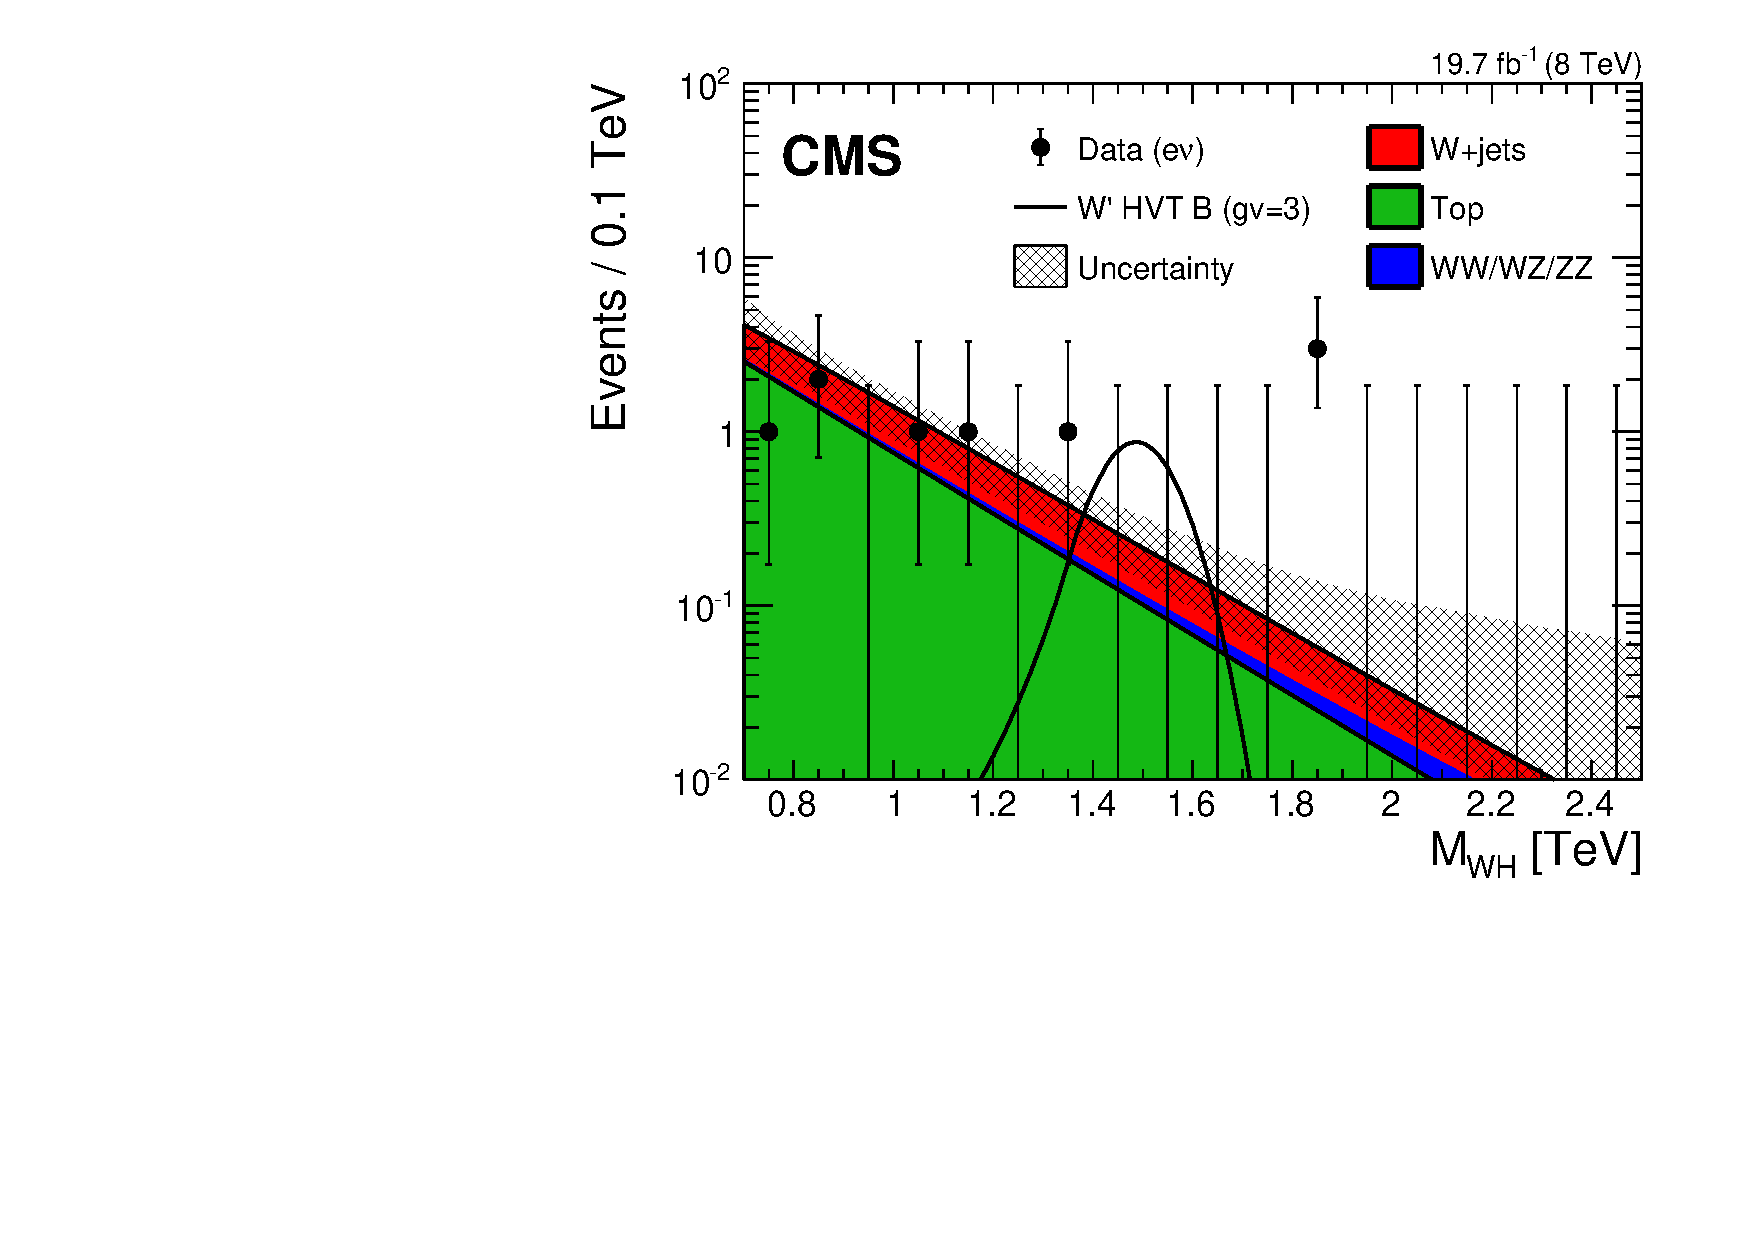
\includegraphics[width=0.45\textwidth]{\chnine/signal-region-el.pdf}}
\subfigure[]{\label{fig:mWH-final_b}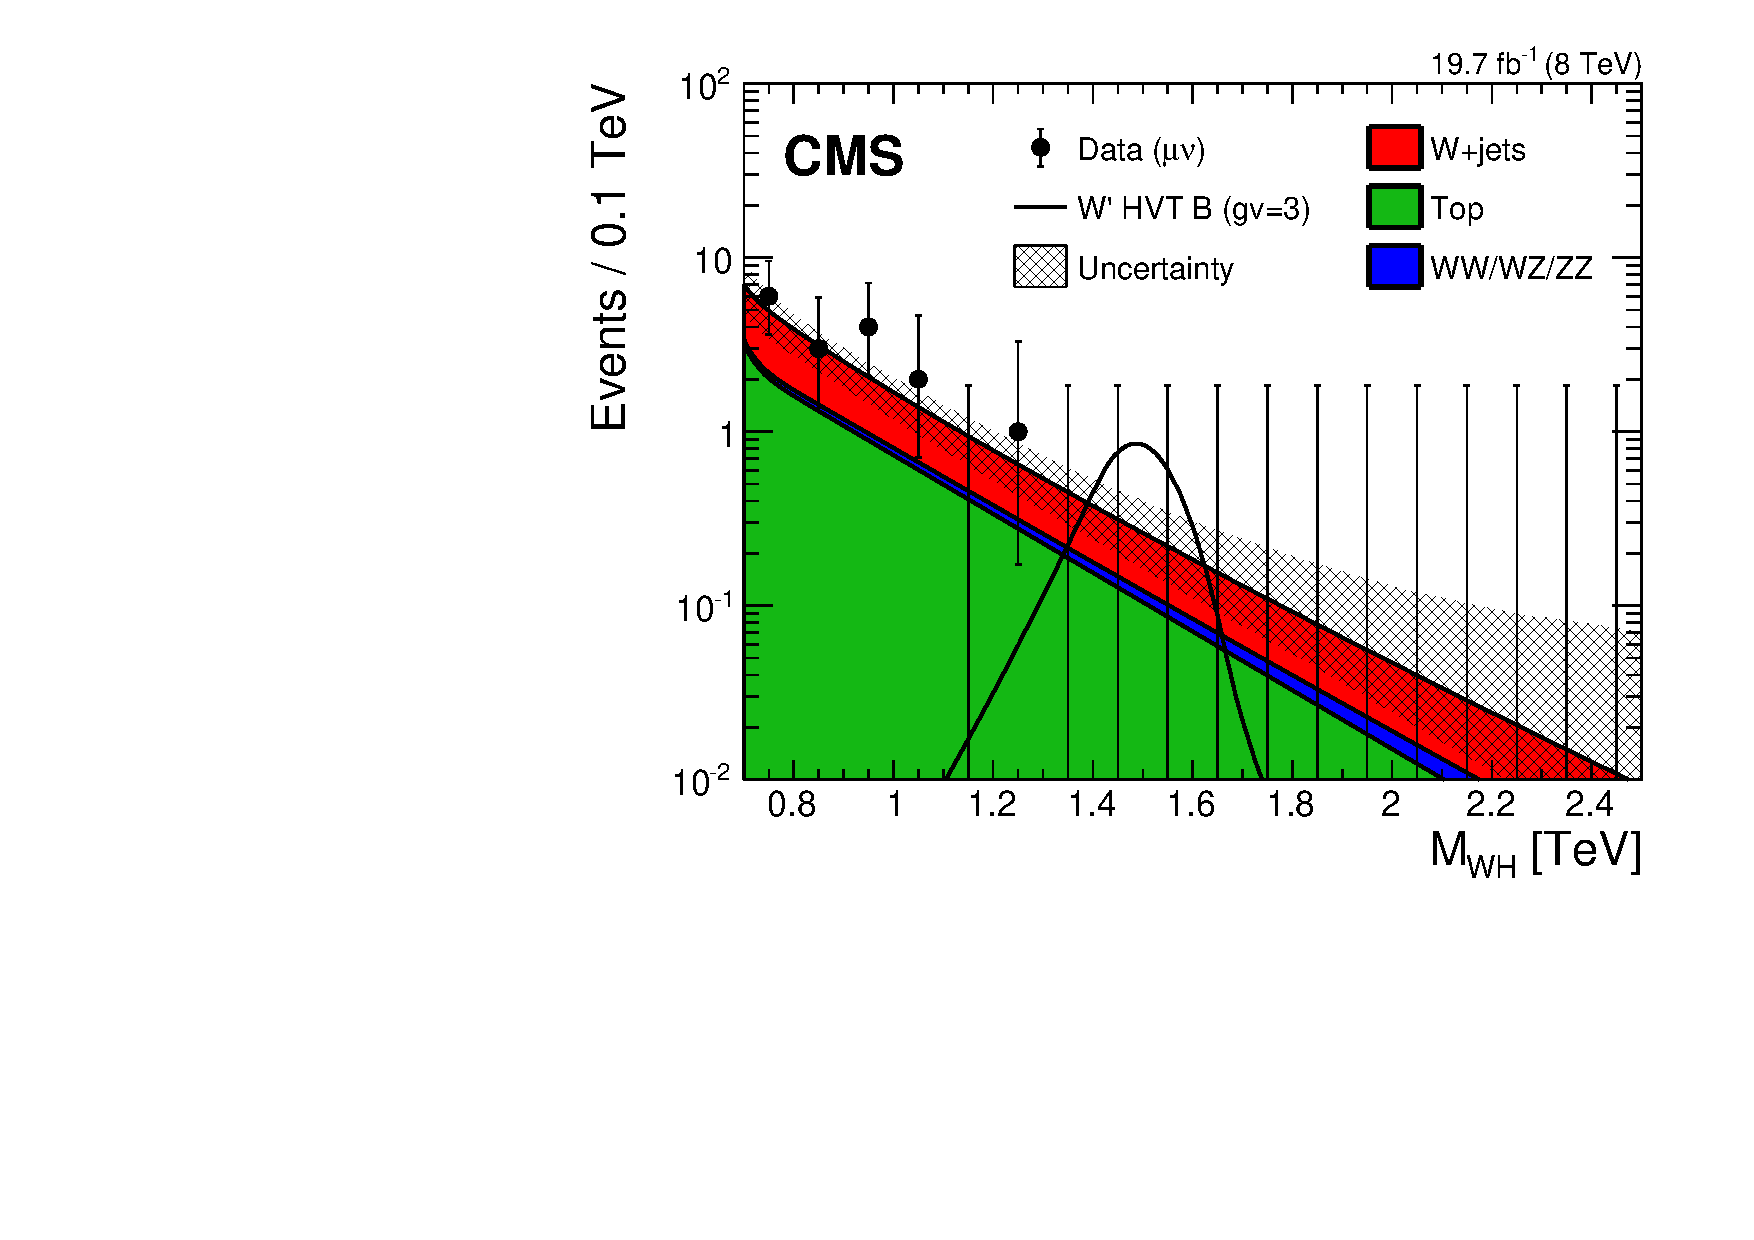
\includegraphics[width=0.45\textwidth]{\chnine/signal-region-mu.pdf}}
\caption{
Final distributions in \mWH for data and expected backgrounds for electron (a) and muon (b) categories.
The 68\% error bars for Poisson event counts are obtained from the Neyman construction~\cite{Garwood}. The hatched region indicates the statistical uncertainty of the fit combined with the systematical uncertainty in the shape. This figure also shows a hypothetical $\PWpr$ signal with mass of 1.5\TeV, normalized to the cross section predicted by the HVT model B with parameter $g_V=3$ as described in Section~\ref{subsec:hvt}.
}
\label{fig:mWH-final}
\end{figure}

%%%%%%%%%%%%%%%%%%%%%%%%%%%%%%%%%
\section{Significance of the data}\label{sec:signif8TeV}
%%%%%%%%%%%%%%%%%%%%%%%%%%%%%%%%%

A comparison between the \mWH distribution observed in data and the largely data-driven
background prediction is used to test for the presence of a resonance decaying into WH.
As described in Section~\ref{sec:stat}, the statistical test is performed based on a profile likelihood discriminant for an unbinned shape analysis.
%Systematic uncertainties in the signal and background yields are treated as nuisance parameters and profiled in the statistical interpretation using log-normal priors,
%while Gaussian priors are used for shape parameters only.
Systematic uncertainties in the signal and background prediction are treated as nuisance parameters and profiled in the statistical.
Uncertainties in the background yield are constrained using log-normal priors, while Gaussian priors are used for uncertainties in the signal and background shape parameters.
Uncertainties in the signal yield are not included in the computation of the p-value.
Systematic uncertainties in the signal and background yields are treated as nuisance parameters and profiled in the statistical interpretation using log-normal priors,
The local significance of the observations is evaluated in the context of the described statistical test,
under the assumptions of a narrow resonance decaying into the WH final state and lepton universality for the W-boson decay, by combining the two event categories.
Correlations arising from the uncertainties common to both channels are taken into account.
The result is shown in Fig.~\ref{fig:sigWH}. The highest local significance of 2.2 standard deviations is found for a resonance mass of 1.8\TeV, driven by the excess in the electron channel described in the previous section.
The corresponding local significance for a resonance of 1.8\TeV in the electron channel is 2.9 standard deviations, while in the muon channel there is no significance.

\begin{figure}[!htb]
\centering
     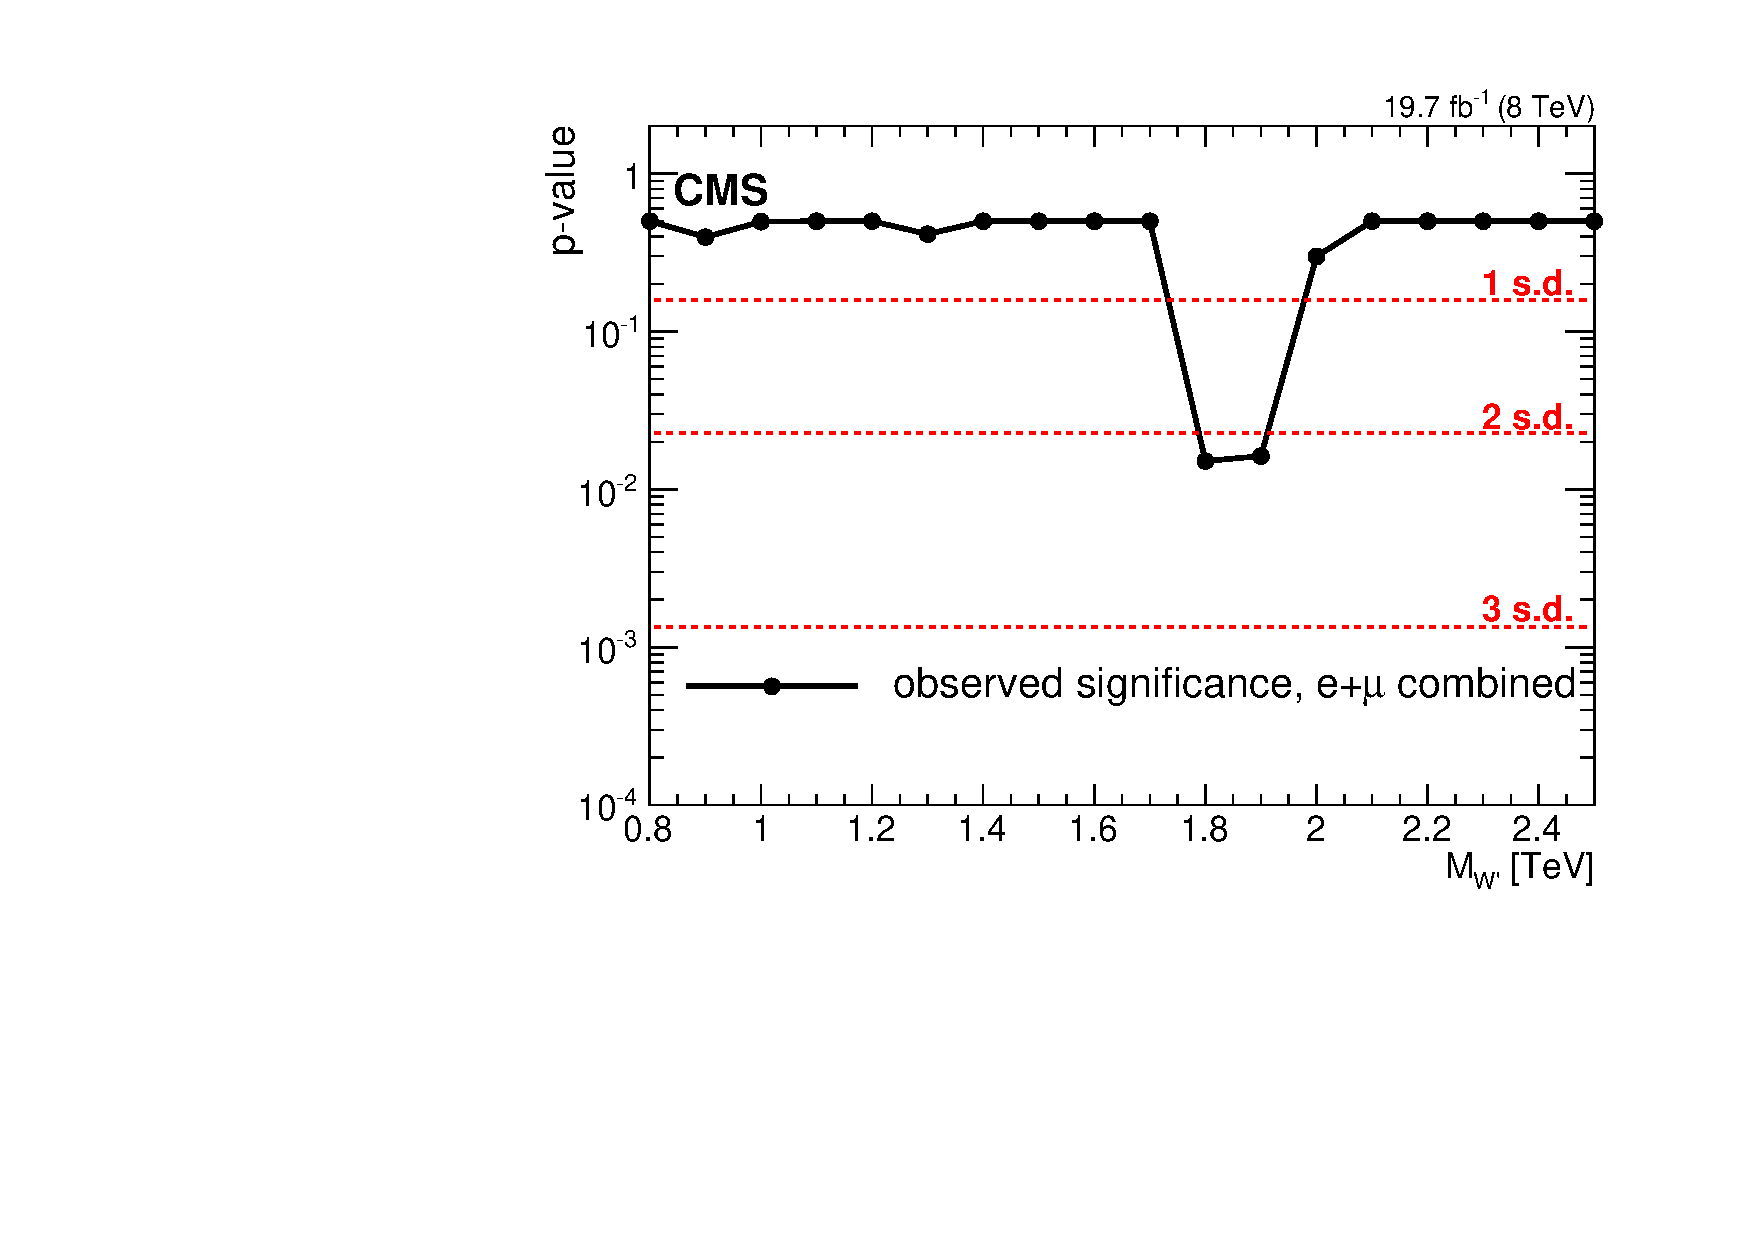
\includegraphics[width=0.45\textwidth]{\chnine/pvalue_combo.pdf}
\caption{
  Local p-value of the combined electron and muon data as a function of the $\PWpr$ boson mass,
  probing a narrow WH resonance.
}
\label{fig:sigWH}
\end{figure}

Taking into account the look-elsewhere effect (Section~\ref{subsec:pvalue}), the local significance of 2.9 standard deviations can be translated into a global significance value by computing the trial factor as given by Eq.~\ref{eqn:trials}. 
Considering the mass range 0.8--2.5\TeV and an average mass resolution of 100\GeV, a trial factor of $\approx$ 16.4 is obtained. The factor, when multiplied by the local p-value, gives a global significance of 1.9 standard deviations
when searching for resonances over the full mass range and across two channels.
In order to cross check this final value, the LEE is also estimated by means of background-only pseudo-experiments. The relation between the global and local significances obtained with this method is shown in Fig.~\ref{fig:sigGlobWH},
and it agrees with the calculation performed with the trial factor.
It can be concluded that the results are thus statistically compatible with the SM expectation within 2 standard deviations.

\begin{figure}[!htb]
\centering
     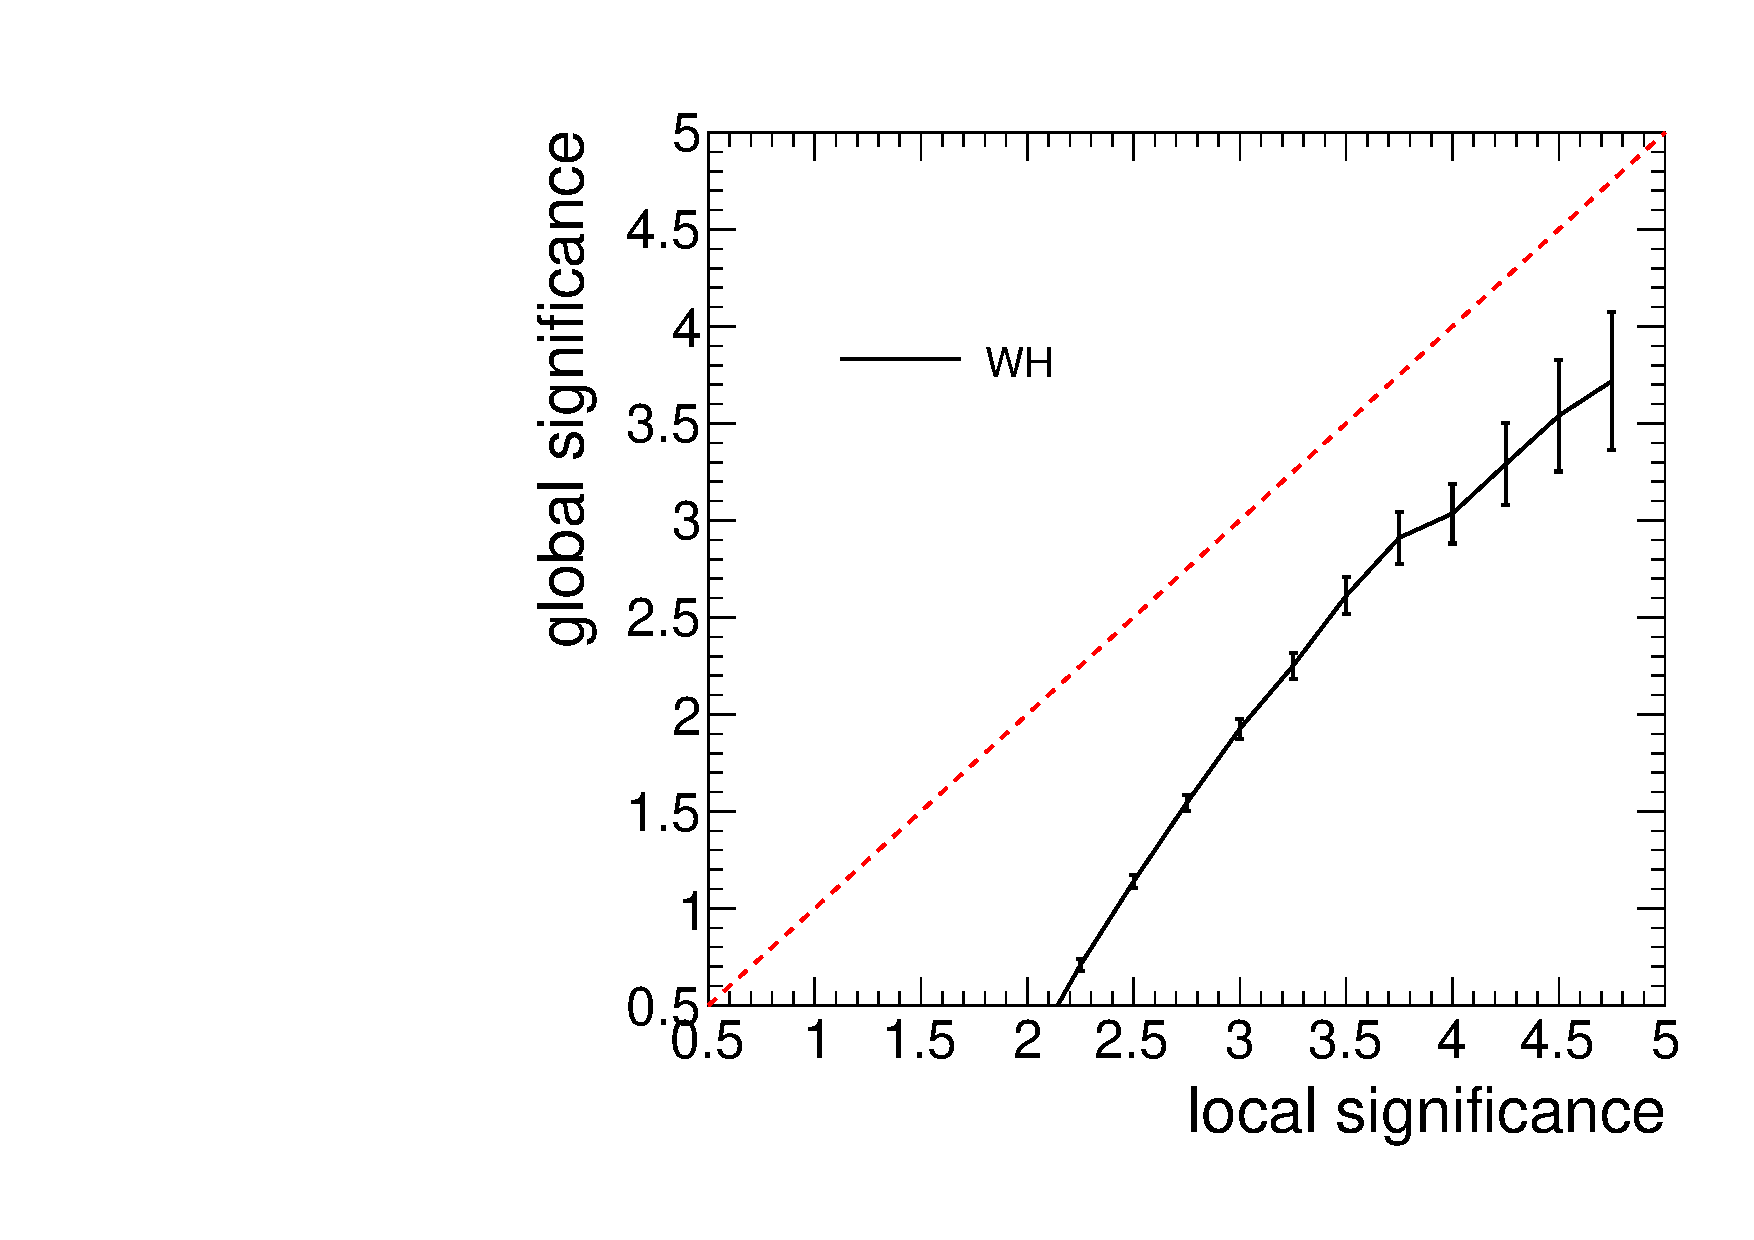
\includegraphics[width=0.45\textwidth]{\chnine/global-vs-local-significance-M800-2500-combo.pdf}
\caption{
  Global significance as a function of the local significance which corresponds to the maximal significance in the \mWH range 0.8--2.5\TeV in the two categories. The global significance is estimated with a frequentist approach using background-only pseudo-experiments and corresponds to the fraction of toys (translated from a p-value to significance) with at least a certain local significance in the \mWH range in the two categories.
}
\label{fig:sigGlobWH}
\end{figure}

%%%%%%%%%%%%%%%%%%%%%%%%%%%%%%%%%
\section{Cross section limits}
%%%%%%%%%%%%%%%%%%%%%%%%%%%%%%%%%

Since no excesses with significance larger than three standard deviations are observed, upper limits are set on the production cross section of the new resonance following the modified-frequentist $\mathrm{CL}_s$ method
described in Section~\ref{sec:stat}. Exclusion limits can be set as a function of the \Wpr resonance mass, under the narrow-width approximation.
The results are interpreted in the HVT model B and in the context of the little Higgs model.\\

Figure~\ref{fig:limitsFullCLS-WH} shows the expected and observed exclusion limits at 95\% CL on the product of the \Wpr production cross section and the branching fraction of $\Wpr\to\PW\PH$ for the
electron and muon channels separately, and for the combination of the two. The limits are compared with the prediction of the two theoretical models.
For the combined channels, the observed and expected lower limits on the $\Wpr$ mass are 1.4\TeV in the LH model and 1.5\TeV in the HVT model B.
For the electron (muon) channel, the observed and expected lower limits on the $\Wpr$ mass are 1.2 (1.3)\TeV in the LH model and 1.3 (1.3)\TeV in the HVT model B.

These results are finally combined with other searches for heavy resonances decaying into diboson performed with pp collisions at 8 and 13\TeV as described in Chapter~\ref{ch:combination}.

 \begin{figure}[!t]
\centering
\subfigure[]{\label{fig:limitsFullCLS-WH_a}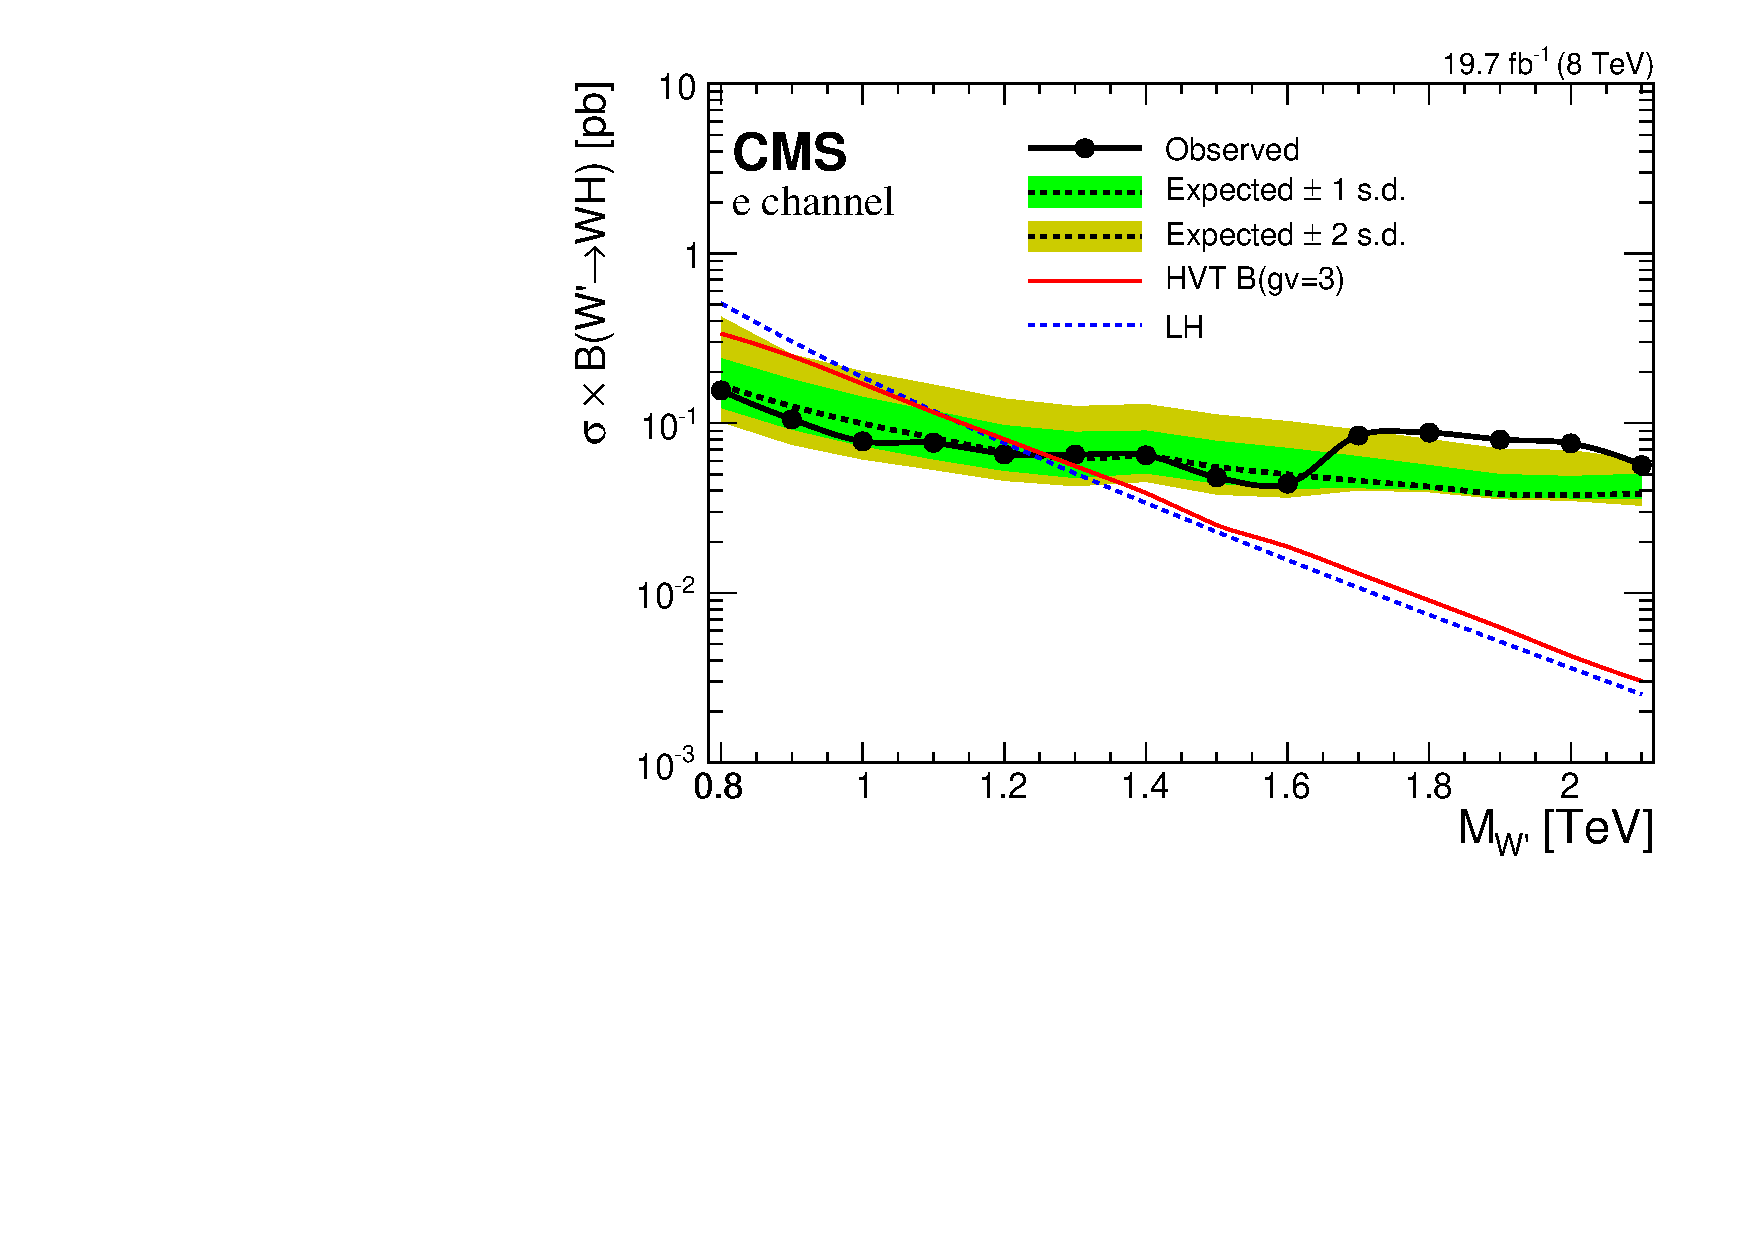
\includegraphics[width=0.45\textwidth]{\chnine/Lim_el_cls.pdf}}
\subfigure[]{\label{fig:limitsFullCLS-WH_b}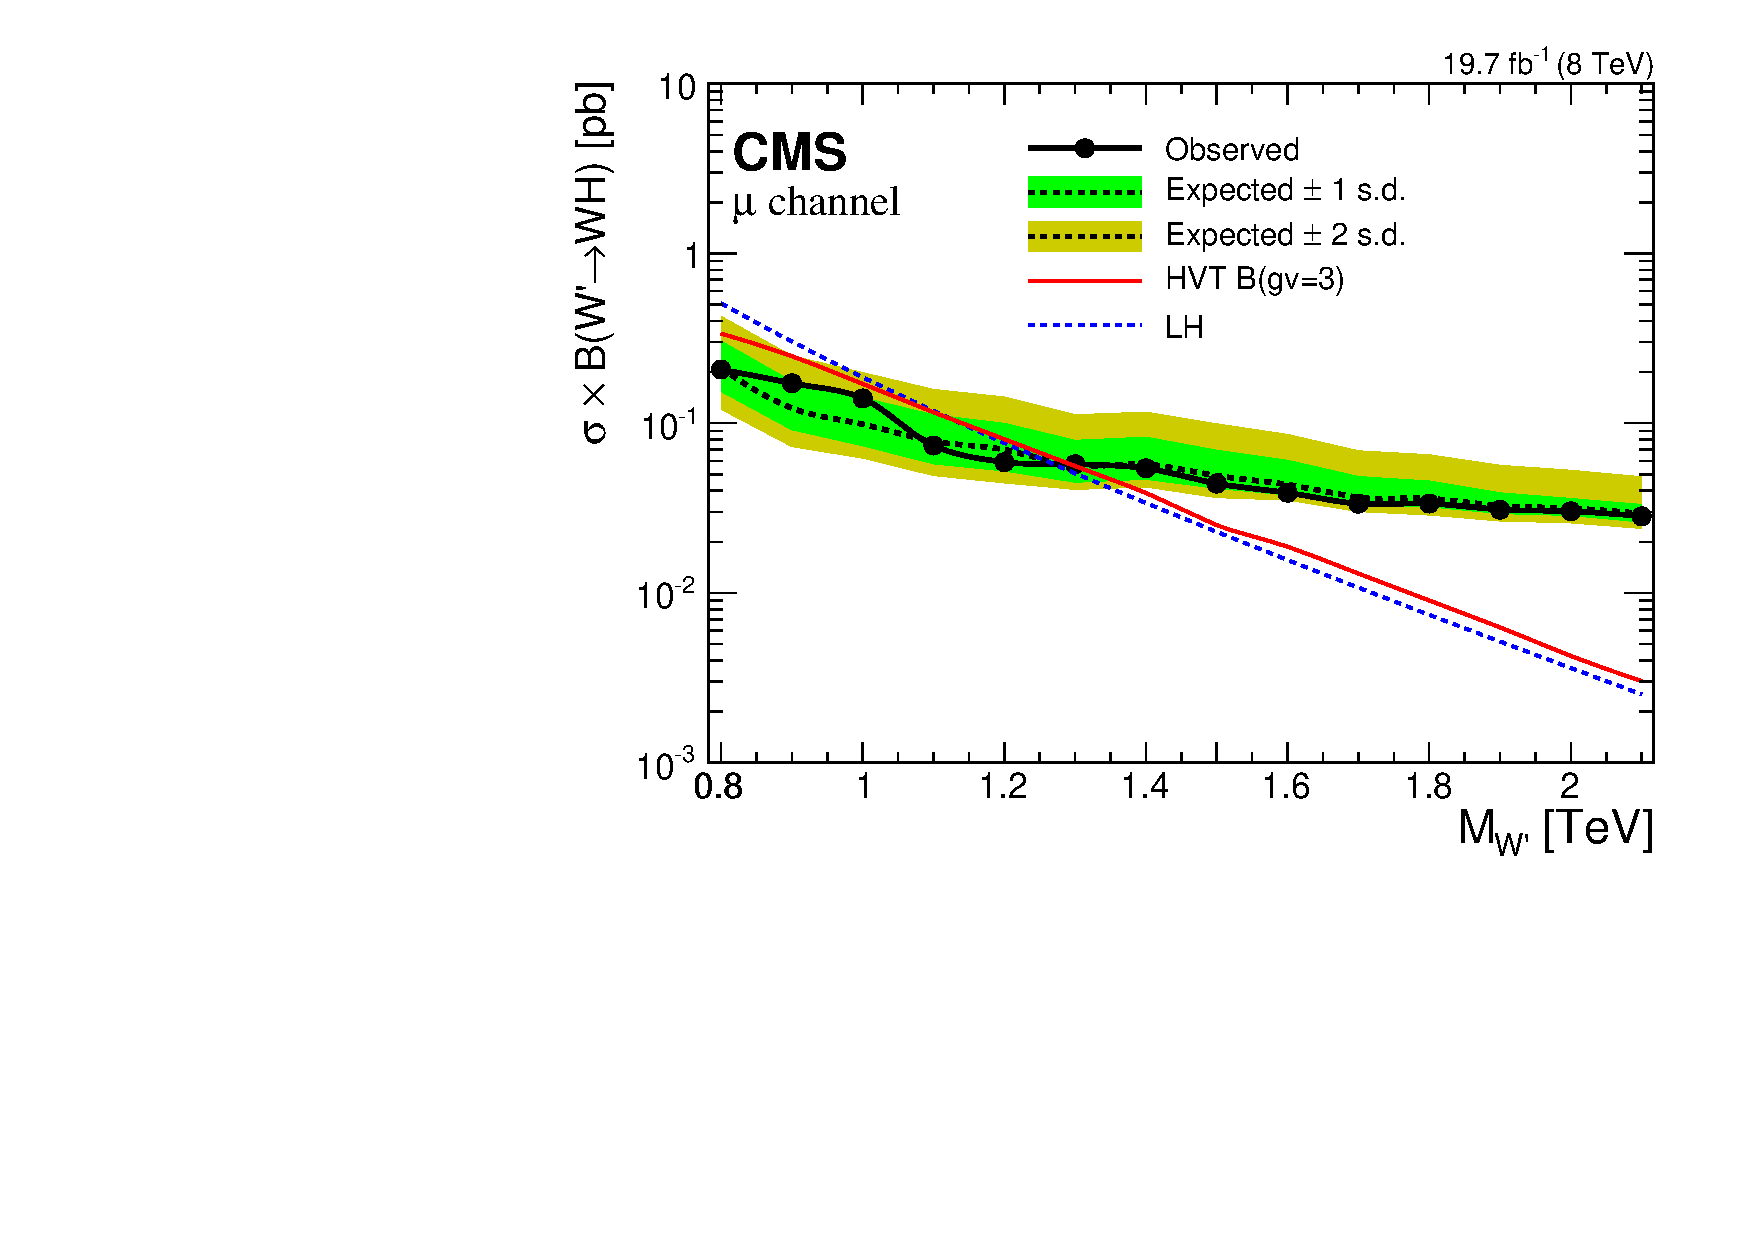
\includegraphics[width=0.45\textwidth]{\chnine/Lim_mu_cls.pdf}}\\
\subfigure[]{\label{fig:limitsFullCLS-WH_c}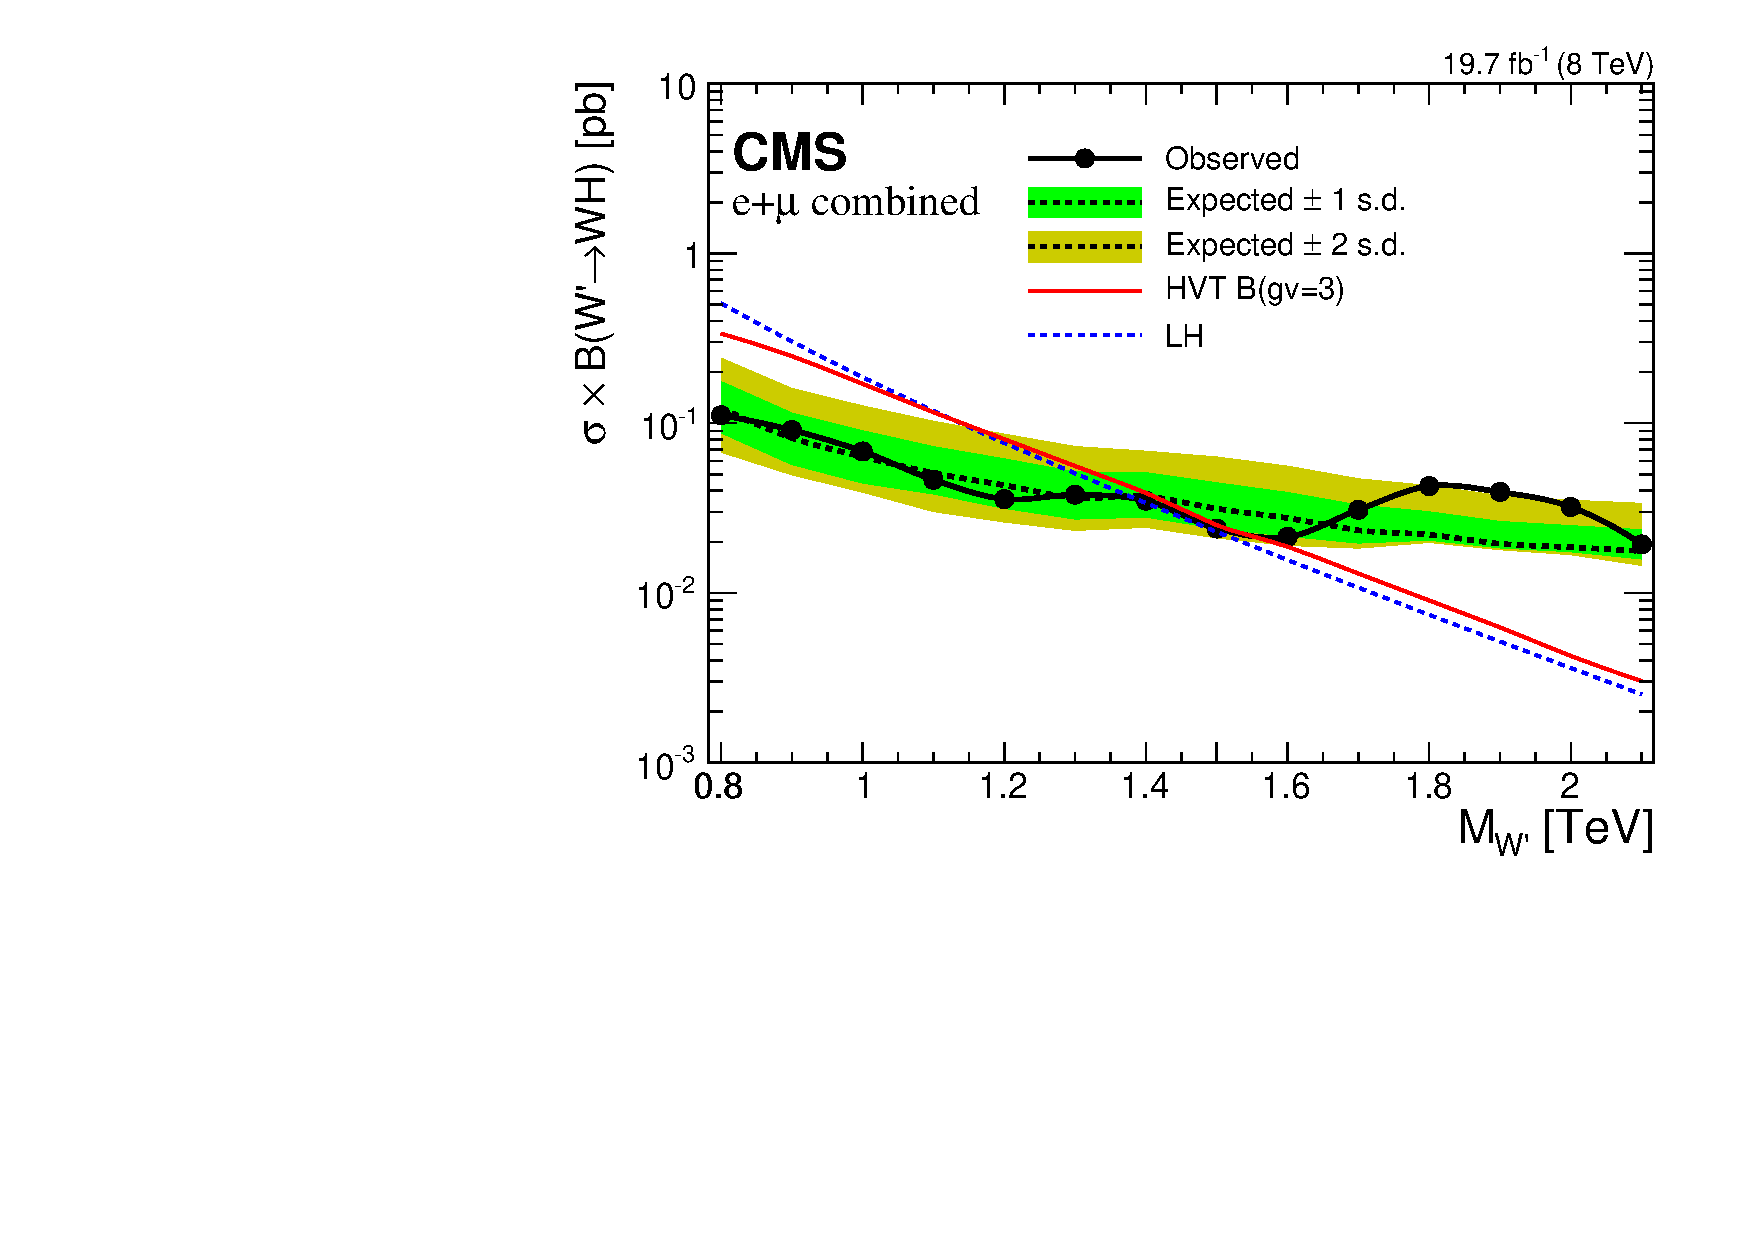
\includegraphics[width=0.45\textwidth]{\chnine/Lim_combo_cls.pdf}}
\caption{
  Observed (solid) and expected (dashed) upper limits at 95\% CL on the
  product of the $\PWpr$ production cross section and the branching
  fraction of $\PWpr\to\PW\PH$ for electron (a) and muon (b) channels,
  and the combination of the two channels (c). The products of cross sections and branching fractions for $\PWpr$ production in the LH and HVT models are overlaid.
}
\label{fig:limitsFullCLS-WH}
\end{figure}